\documentclass[border=2pt]{standalone}
\usepackage{tikz}
\begin{document}
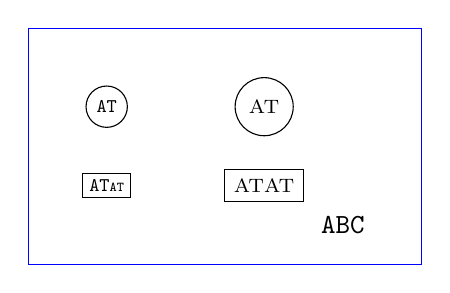
\begin{tikzpicture}[font=\ttfamily]
  \draw[blue,line width=.2pt] (-1,-1) rectangle (4,2);
  \node[scale=.7,draw] at (0,0) {AT{\scriptsize AT}};
  \node[font=\scriptsize,draw] at (2,0) {AT{\scriptsize AT}};
  \node[scale=.7,draw,circle,minimum size=10pt] at (0,1) {AT};
  \node[font=\scriptsize,draw,circle,minimum size=10pt] at (2,1) {AT};
  \node at (3,-.5) {A\textbf{B}C};
\end{tikzpicture}
\end{document}
